%==============================================================================
% Sjabloon poster bachproef
%==============================================================================
% Gebaseerd op document class `a0poster' door Gerlinde Kettl en Matthias Weiser
% Aangepast voor gebruik aan HOGENT door Jens Buysse en Bert Van Vreckem

\documentclass[a0,portrait]{hogent-poster}

% Info over de opleiding
\course{Bachelorproef}
\studyprogramme{toegepaste informatica}
\academicyear{2022-2023}
\institution{Hogeschool Gent, Valentin Vaerwyckweg 1, 9000 Gent}

% Info over de bachelorproef
\title{Strategieën om de overname van bestaande webshops naar WordPress met WooCommerce te stroomlijnen: een onderzoek en proof-of-concept.}
%\subtitle{Ondertitel (eventueel)}
\author{Bjorn Truye}
\email{bjorn.truye@student.hogent.be}
\supervisor{Sofie Lambert}
\cosupervisor{Dennis Matthijs (Team Made)}

% Indien ingevuld, wordt deze informatie toegevoegd aan het einde van de
% abstract. Zet in commentaar als je dit niet wilt.
\specialisation{Mobile \& Enterprise developer}
\keywords{Webapplicatieontwikkeling; Webdevelopment; CMS; Webshop}
\projectrepo{https://github.com/TBthe1/2022-2023-bachelorproef}

\begin{document}

\maketitle

\begin{abstract}
    Een webshop overnemen vereist enige programmeerkennis. Er kunnen veel (externe) factoren zorgen voor een moeilijke overdracht. Klanten moeten hun eigen webshop zelf kunnen beheren, een webshop kan een ingewikkelde lay-out hebben, er kunnen al veel artikelen aanwezig zijn enzovoort. Hoe kunnen we een overname zo eenvoudig en minst tijdrovend mogelijk maken?
\end{abstract}

\begin{multicols}{2} % This is how many columns your poster will be broken into, a portrait poster is generally split into 2 columns

\section{Introductie}
Een webshop is een website waarop goederen en/of diensten worden verkocht. Om een webshop van inhoud te voorzien moet deze zo eenvoudig mogelijk opgevuld worden. Hiervoor bestaan er verschillende tools, waaronder een CMS of contentmanagementsysteem. Hiermee kan door een inlogsysteem de klant de webshop bewerken, zonder enkele programmeerkennis. Team Made gebruikt hiervoor WordPress. Standaard is WordPress maar een website voor blogberichten. Via uitbreidingen op deze tool, bekent onder de naam plugins, kan er zo een webshop worden gemaakt. Een bekende plugin die Team Made hiervoor gebruikt is WooCommerce. 
\\\\
Het overnemen van een webshop betekent dat je een nieuwe webshop maakt, en zo veel mogelijk van de originele webshop probeert over te nemen. Idealiter worden problemen of mankementen bij een overname niet erbij betrokken. Voor Team Made betekent dit een nieuwe WordPress met WooCommerce opzetten, en zo veel mogelijk proberen over te nemen van de originele webshop.

\section{Experimenten}

Omdat er veel verschillende scenario’s mogelijk zijn voor een overname van een webshop, zal een stappenplan worden opgesteld. Dit stappenplan zal als korte leidraad
dienen. Het doel hiervan is om zo veel mogelijk stappen geautomatiseerd te hebben. Afhankelijk van het scenario kunnen hierbij stappen overgeslaan worden. Zo is het bv. overbodig om een databank aan te maken als er al één voorzien is. 
\\\\
De hele opzet van WordPress kan geautomatiseerd worden met behulp van scripts, maar is niet altijd voordelig. Het overnemen van bestaande webshops hun designs en data kan verwezenlijkt worden door een combinatie van manueel programmeerwerk en AI-tools te gebruiken.

%\section{Sectie met figuur}
%
%De {\LaTeX} figure-omgeving bepaalt zelf waar een afbeelding komt en dat is meestal niet op de plek in de tekst waar de figure-omgeving gedefinieerd wordt. Als je wilt forceren dat afbeeldingen toch in de flow van de tekst blijven, dan kan je dat zoals hieronder:
%
\begin{center}
  \captionsetup{type=figure}
  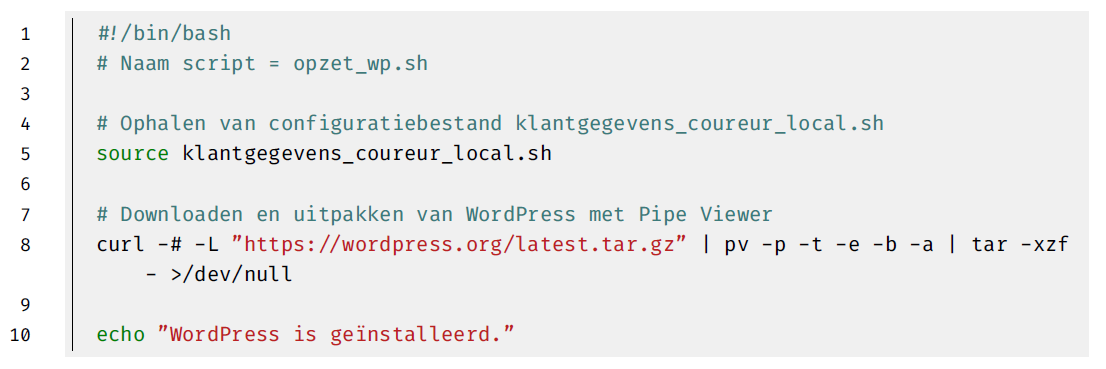
\includegraphics[width=1.0\linewidth]{opzet_wp}
  \captionof{figure}{Opzet van laatste WordPress-versie automatiseren met een configuratiebestand met Bash}
\end{center}
%
%Let er wel op dat dit tot problemen met bladschikking kan leiden.

\section{Conclusies}
De verwachtingen zijn dat er enorm veel AI-tools gaan blijven bijkomen om niet alleen het leven van de programmeurs, maar ook andere jobs te vereenvoudigen.
Dat er één AI-tool zal ontstaan die de volledige opzet, opvulling, onderhoud en het online zetten van een webshop op zich kan nemen, lijkt zeer realistisch en niet meer zo veraf te zijn. Er is nog steeds een expert nodig die begrijpt wat er allemaal aan het gebeuren is. Niet alleen om de noodzakelijke aanpassingen uit te voeren, maar ook omdat het concept van automatiseren met AI nog steeds veel manuele input vergt.
\\\\
Van zodra image-recognition in AI-tools voor iedereen toegankelijk wordt dan gaat het overnemen van een bestaande webshop gigantisch snel gaan. Screenshots
kunnen nemen van een design, en vragen om dit in code uit te schrijven, gaat enorm veel tijd besparen. Op moment van schrijven kan dat nog niet en moet
de gebruiker zeer gedetailleerd beschrijven wat hij van code wenst te ontvangen.

\section{Toekomstig onderzoek}
Elementor AI zal hoogstwaarschijnlijk een interessante optie zijn voor Team Made, die heel wat zaken van een webshop overname kan automatiseren. Het is sterk aangeraden om hiermee te experimenteren van zodra het product publiek toegankelijk is. Probeer in het algemeen zoveel mogelijk verschillende AI-tools uit, en bekijk welke de beste resultaten specifiek voor een bepaald project opleveren. Dezelfde vraag in tool A kan een volledig ander resultaat opleveren in tool B. Blijf het aanschouwen als een hulpmiddel, en niet als een volledig vervangmiddel.
\end{multicols}
\end{document}